\documentclass{article}
\usepackage[utf8]{inputenc}
\usepackage{amsmath, amssymb}
\usepackage{amsthm}
\usepackage{graphicx}
\usepackage{enumitem}
\usepackage{titlesec}
\usepackage[hidelinks]{hyperref}
\usepackage{geometry}
\geometry{margin=1in}
\usepackage[T1]{fontenc}
\usepackage{lmodern}
\usepackage{tabularx}
\usepackage{booktabs}
\usepackage{array}
\usepackage{float} 
\usepackage[round]{natbib}
\usepackage{setspace}
\usepackage{booktabs}
\usepackage[table]{xcolor}
\setstretch{1.5}  


\title{Belonging and Drift:\\ An Agent-Based Model of Lesbian Space Transformation}
\author{Wendi Xue}
\date{} 

\begin{document}

\maketitle

\textbf{GitHub Link:} \url{https://github.com/wendixue/lesbian_bar_abm_wendix/tree/Wendy-Branch}

\section{Introduction}

\indent

In recent years, the decline of lesbian bars has accelerated due to the growing influence of digital dating platforms and the changing patterns of queer social life. These bars, which once played a central role in fostering lesbian community and cultural identity, are increasingly struggling to remain open. In order to survive, many have adopted new strategies by expanding their target clientele to include all queer individuals or all women. Although these changes are often framed as efforts to promote inclusion, they have also raised concerns about the erosion of lesbian-specific spaces and the weakening of lesbian cultural identity.

This project investigates how lesbian bars adapt to these pressures and what consequences follow from their strategic decisions. The central research question is: \textbf{How do differences in strategic orientation and adaptive capacity among lesbian bars shape their evolving clientele and cultural atmosphere over time?}

To answer this question, the study addresses two sub-questions:
\begin{enumerate}
    \item How do different strategic orientations (woman-centered vs. queer-centered) of lesbian bars influence the demographic composition and cultural character of these spaces over time?
    \item How does a bar’s level of adaptive responsiveness affect the demographic composition and cultural character of these spaces over time?
\end{enumerate}

Together, these questions reflect a broader interest in how identity-based spaces, such as lesbian bars, respond to external cultural and economic pressures. They aim to clarify how such spaces negotiate the tension between expanding their reach and preserving a distinct cultural identity. By focusing on lesbian bars as a case, this project seeks to illuminate the mechanisms through which strategic orientation and adaptive responsiveness shape both the composition of their clientele and the evolution of their cultural atmosphere over time.

\section{Literature Review}

\indent

Lesbian bars have historically functioned as culturally bounded spaces that prioritize the safety, intimacy, and solidarity of queer women. These boundaries, often maintained by restricting access to non-women and non-lesbian patrons, were central to the construction of lesbian social identity and political cohesion \citep{podmore2006}. However, in recent years, many lesbian bars have altered their inclusion strategies in response to economic pressure, urban transformation, and evolving social norms around gender and sexuality. Two dominant orientations have emerged: woman-centered bars, which extend access to all women regardless of sexual identity, and queer-centered bars, which welcome a wider spectrum of LGBTQ+ individuals, including queer non-women \citep{mattson2023, browne2021}.



Although these strategies are often framed as inclusive and necessary for survival, they have raised concerns about the dilution of lesbian-specific cultural identity. \citet{mattson2023} describes how financial rebranding can prompt patrons to disengage when they no longer recognize a space as culturally lesbian. \citet{podmore2006} documents how the inclusion of mixed-gender participation in formerly women-only venues can reduce lesbian visibility and weaken symbolic cohesion. \citet{browne2021} critiques the broader erasure of ``lesbian'' as a distinct spatial and political category within generalized LGBTQ+ frameworks.


These accounts directly inform the model’s first design feature: bar-level strategic orientation, which influences how different inclusion strategies affect the composition and symbolic identity of lesbian spaces over time.

However, formal inclusion policies alone do not determine how patrons relate to a space. Spatial belonging is not merely about access; it is shaped by affective evaluation, perceived fit, and cultural resonance. \citet{held2009} demonstrates that individuals from different identity positions may interpret the same environment in contrasting ways. Even in venues that claim inclusivity, patrons may experience cultural dissonance or misalignment with dominant norms. This insight supports the model’s second key mechanism: individual-level evaluations of belonging influence whether patrons stay, leave, or return to a space.

Belonging is further shaped by interaction and emotional context. \citet{baxter2024} argue that lesbian nightlife is defined less by fixed locations and more by affective spatialities—emotional atmospheres created through shared experiences and social dynamics. In this perspective, belonging is not simply an outcome of identity alignment, but an emergent judgment tied to the immediate social and cultural conditions of a space. Building on this view, the model treats belonging as a round-based evaluation, influenced by each agent’s most recent interaction with a space. Rather than storing long-term memory, agents update their willingness to return based on the latest experience, reflecting how real-world participation is often guided by recent impressions.

Collectively, these studies suggest that individual perceptions of cultural fit, shaped by both institutional signals and peer dynamics, play a central role in sustaining or eroding lesbian spaces. As patrons assess their sense of belonging and adjust their participation accordingly, their choices alter the demographic and cultural composition of the space. This recursive relationship between individual experience and space-level transformation constitutes the central feedback mechanism this project seeks to theorize and formalize.

While these literatures provide rich accounts of how individuals interpret and navigate lesbian spaces, they remain largely focused on the micro-level. They excel at describing identity negotiation, affective response, and localized inclusion and exclusion, but offer limited tools for analyzing how individual decisions accumulate over time to produce institutional and cultural change. To address this gap, this project employs an agent-based model that simulates how patterns of bar selection, withdrawal, and belonging evolve under different institutional strategies. By modeling the feedback loop between agents’ subjective evaluations and the changing cultural profile of each bar, the model offers a structural and process-based account of how lesbian spaces retain, transform, or lose their cultural identity in the face of strategic adaptation.

\section{Theoretical Causal Mechanism}

This project models a feedback loop between individual experiences of belonging and the cultural evolution of lesbian bars. It examines how patrons, guided by identity-specific sensibilities, respond to both institutional strategies and social atmospheres, and how these responses, in turn, reshape the identity of the space over time.

At the individual level, each agent evaluates their subjective sense of belonging within a bar. This belonging score is shaped by three key inputs: the bar’s fixed structural orientation, which encodes its baseline affinity for different identity groups; the bar’s adaptive cultural tone, which reflects the recent composition of patrons and signals the emergent atmosphere of the space; and the agent’s preferences regarding co-presence with other identity groups. These inputs are combined into a single judgment that reflects how well a space aligns with the agent’s identity, expectations, and sense of social comfort.

This evaluation is immediate and updated each round. If the belonging score exceeds the agent’s threshold, they choose to attend or remain in the bar. If it falls short, they withdraw, either temporarily or permanently after repeated misalignment. In this way, belonging is modeled not as a binary state but as a dynamic, identity-contingent outcome shaped by spatial structure and group composition.

At the macro level, bars differ in both their strategic orientation and their degree of social adaptability. All bars center queer women as their primary audience, but they differ in how they relate to adjacent groups. Woman-centered bars assign higher baseline affinity to all women, including non-queer women. Queer-centered bars assign higher affinity to queer individuals who are not women. These two orientations represent distinct ways of extending inclusion beyond the lesbian core, either through shared gender identity or through broader queer affiliation.

Bars also differ in their social adaptability, defined as the extent to which their adaptive affinity influences their overall cultural profile. Bars with high adaptability place greater weight on recent attendance patterns, making their effective affinity more sensitive to social feedback. Bars with low adaptability rely more heavily on their fixed baseline structure, maintaining cultural stability but responding more slowly to change. This adaptability is not a matter of how frequently bars update, but of how much influence recent participation has on the cultural signals a bar produces.

Together, these dynamics form a recursive feedback loop. Bars generate different belonging scores for different patrons, based on their strategic settings and recent visitor composition. Patrons respond to these belonging scores by deciding whether to participate. Their collective presence, in turn, reshapes the demographic and cultural atmosphere of the bar, influencing how welcoming it appears to different groups in subsequent rounds. Over time, this feedback process can reinforce a coherent lesbian cultural identity, facilitate gradual diversification, or lead to symbolic erosion.

This model provides a process-based account of how lesbian bars evolve through the interaction of institutional design, affective experience, and social participation. It demonstrates how symbolic identity is continually reconstructed through patterns of inclusion and exclusion, not only through who is formally allowed into a space, but through who feels they belong, chooses to stay, and collectively sustains the cultural character of that space.

\section{Model Overview}

This agent-based model simulates the dynamic interaction between individual patrons and lesbian bars. It includes two types of agents: customer agents, representing individuals with diverse identities and belonging thresholds; and bar agents, representing physical venues with fixed strategic orientations and varying levels of cultural adaptability. 

\subsection{Model Components}

\subsubsection{Customer Agents}

Customer agents (\textit{PersonAgent}) represent potential lesbian bar patrons who differ in identity, sensitivity to exclusion, and subjective experiences of belonging. Each agent is assigned to one of three identity groups, which shape both how they interpret space and how they are received by it. In the model's baseline configuration, the population is initialized with the following proportions:

\begin{itemize}
    \item QW (Queer Women) – 50\% of agents
    \item NQW (Non-Queer Women) – 25\% of agents
    \item QNW (Queer Non-Women) – 25\% of agents
\end{itemize}

These identity positions determine how agents respond to the social and cultural atmosphere of each bar. Agents do not assess space in abstraction; instead, they generate a belonging score for each bar based on two components: (1) how welcoming the bar appears structurally and culturally toward their identity, and (2) how comfortable they feel in relation to the current patrons. 

Each agent is initialized with the following psychological attributes:

\begin{itemize}
    \item \textbf{Belonging threshold:} This defines the minimum belonging score required for an agent to consider entering a bar. It captures individual sensitivity to exclusion. In the current model, each agent is assigned a value randomly drawn from a normal distribution between 0.4 and 0.6. This value remains fixed for each agent throughout the simulation.
    \item \textbf{Intergroup preference profile:} This defines how positively or negatively an agent evaluates the presence of each identity group in a bar. The model uses a predefined intergroup preference matrix that sets baseline values for how each group relates to others. Each agent samples their preferences from a normal distribution centered at the group-level baseline, with variation drawn from a ±0.1 range. These preferences are asymmetric and identity-specific, and were constructed based on qualitative syntheses of existing literature and social media discussions on inclusion and discomfort in queer nightlife.
\end{itemize}

At any point in the simulation, agents can be in one of three states:
\begin{itemize}
    \item \textbf{Active}: Participating in bar selection and attendance
    \item \textbf{Temporarily exited}: Withdrawn due to unmet belonging conditions, with the potential to return after a randomly assigned period between 5 and 15 rounds
    \item \textbf{Permanently exited}: Removed from the simulation after two repeated unsuccessful attempts to find a bar that meets their threshold
    
\end{itemize}

\subsubsection{Bar Agents}

Each bar agent represents a physical venue with a predefined cultural orientation, expressed through its affinity profile toward three identity groups: queer women (QW), non-queer women (NQW), and queer non-women (QNW).

The model includes two types of bars:

\begin{itemize}
    \item Woman-centered bar: Assigns the highest baseline affinity to QW, moderate affinity to NQW, and lower affinity to QNW. This strategy prioritizes shared gender and sexual identity, and reflects a commitment to centering women—especially queer women—as the core constituency.
    \item Queer-centered bar: Also assigns the highest affinity to QW, but allocates moderate affinity to QNW and lower affinity to NQW. While still centering QW, this strategy shifts toward broader queer inclusion across gender identities, including patrons who do not identify as women.
\end{itemize}

Each bar's orientation is encoded in two forms of affinity toward identity groups:

\begin{itemize}
    \item Fixed affinity refers to the bar’s baseline structural orientation. It remains constant over time and reflects the bar’s foundational strategy regarding which groups it is designed to support. In both types of bars, fixed affinity values are assigned on a three-level scale: 1.0 for the most prioritized group, 0.7 for moderate inclusion, and 0.2 for the least prioritized group. For example, a woman-centered bar assigns 1.0 to QW, 0.7 to NQW, and 0.2 to QNW; a queer-centered bar assigns 1.0 to QW, 0.7 to QNW, and 0.2 to NQW.
    \item Adaptive affinity represents the bar’s emergent cultural atmosphere. It is recalculated at regular intervals based on the recent composition of patrons and captures soft, socially constructed dimensions of inclusion—such as collective norms, behavioral tone, word-of-mouth reputation, and emotional resonance. Adaptive affinity evolves gradually in response to who actually attends and shapes the perceived ambiance of the space.
\end{itemize}

\textbf{Adaptive Affinity:}
\[
\text{Adaptive Affinity}_g = \frac{\#\text{group } g \text{ visitors in recent rounds}}{\text{Total visitors in recent rounds}}
\]

where $g \in \{\text{QW}, \text{NQW}, \text{QNW}\}$, and the time window length is determined by a global update interval parameter.

The effective affinity that determines how agents experience a bar is calculated as a weighted average of fixed and adaptive components:

\textbf{Effective Affinity:}
\[
\text{Effective Affinity}_g = \gamma \cdot \text{Fixed Affinity}_g + (1 - \gamma) \cdot \text{Adaptive Affinity}_g
\]

The parameter $\gamma$ governs the degree of social adaptability. Bars with higher $\gamma$ values rely more heavily on their fixed structural identity, while bars with lower $\gamma$ values are more responsive to recent attendance patterns and social feedback. This weighting mechanism allows bars to vary in how stable or fluid their cultural tone becomes over time.


By combining long-term strategic orientation with short-term social responsiveness, this framework allows the model to simulate how lesbian bars either sustain, transform, or lose their symbolic identity through everyday processes of participation and interaction.

\subsubsection{Agent Action Logic}

The simulation progresses in discrete time steps. At each step, all customer agents follow a three-phase decision process: evaluation, decision, and participation and feedback. This process governs their interaction with the bar environment and drives the emergence of system-level cultural patterns.

\paragraph{Belonging Score Calculation}

Each agent computes a belonging score for each bar, formally defined as:

\[
\text{Belonging Score} = \alpha \times \text{Effective Affinity} + (1 - \alpha) \times \text{Peer Comfort}
\]

Where:

\begin{itemize}
    \item \textbf{Effective Affinity} is the bar’s receptiveness toward the agent’s identity group, combining fixed and adaptive components;
    \item \textbf{Peer Comfort} reflects how aligned the current social atmosphere is with the agent’s identity preferences;
    \item $\alpha$ is a global parameter that determines the relative weight of structural versus social cues, set to $0.5$ by default.
\end{itemize}

\paragraph{Peer Comfort Calculation}

Peer comfort is calculated as a weighted average of the agent’s preference toward each identity group present in the bar:

\[
\text{Peer Comfort} = \sum (p_g \times w_g)
\]

Where:

\begin{itemize}
    \item $g \in \{\text{QW}, \text{NQW}, \text{QNW}\}$;
    \item $p_g$ is the proportion of patrons from group $g$ in the bar;
    \item $w_g$ is the agent’s preference weight for group $g$, drawn from a normal distribution centered around a group-specific baseline, with a variation of $\pm 0.1$.
\end{itemize}

This structure allows agents to evaluate space not only by formal inclusivity but also by how socially and emotionally resonant the space feels to them.

\subsubsection*{3.1 Evaluation}

In this phase, each active agent computes belonging scores for both bars using the formula above. The resulting scores capture both institutional design and the current demographic composition of each bar.

\subsubsection*{3.2 Decision}

Agents make entry decisions based on how their computed scores compare to their individual belonging threshold:

\begin{itemize}
    \item If both bars exceed the threshold, the agent selects between them probabilistically, weighted by their relative scores.
    \item If only one bar exceeds the threshold, the agent chooses that bar.
    \item If neither bar meets the threshold, the agent temporarily exits for a random period between $5$ and $15$ rounds.
    \item If an agent experiences two consecutive rounds in which no bar exceeds their threshold, they are permanently removed from the simulation.
\end{itemize}

\subsubsection*{3.3 Participation and Feedback}

Agents who enter a bar contribute to its group composition, influencing the peer comfort of others in the same round. Over time, the presence of different identity groups also affects the bar’s adaptive affinity.

At fixed intervals, each bar updates its adaptive affinity by recalculating the average representation of each group in recent rounds. This models how cultural tone and perceived inclusiveness evolve not through explicit policy change but through cumulative participation patterns.


In addition to their fixed inclusion strategies, bar agents implement a dynamic mechanism of adaptive affinity, allowing them to gradually adjust their cultural orientation based on the identities of recent participants. This models how real-world venues evolve not through formal policy changes, but through subtle shifts in atmosphere and cultural signaling shaped by attendance patterns.

Each bar maintains a history of recent visitors and periodically updates its adaptive affinity profile. The timing of these updates is controlled by the global parameter $adaptive_update_interval$, which determines how frequently each bar incorporates social feedback. At each scheduled interval, the bar calculates the proportion of each identity group among its recent attendees. These proportions form the new adaptive affinity values, reflecting how welcoming the bar is perceived to be based on recent participation rather than institutional intent.



The final effective affinity that agents use to evaluate belonging is computed as a weighted average of the fixed and adaptive components:

\[
\text{Effective Affinity}_g = \gamma \times \text{Fixed Affinity}_g + (1 - \gamma) \times \text{Adaptive Affinity}_g
\]


Here, $\gamma$ is a global parameter that governs the bar’s social adaptability. A higher gamma places more weight on fixed affinity, making the bar culturally stable and resistant to change. A lower gamma places more weight on adaptive affinity, making the bar more responsive to short-term patterns of participation.

Through this mechanism, the model captures how institutional identity evolves through social feedback rather than top-down redesign. It provides a formal structure for simulating how repeated attendance patterns influence the long-term cultural trajectory of lesbian bar spaces—either reinforcing a coherent identity or enabling symbolic drift over time.

\section{Analysis}

\subsection{Cultural Pathways and the Limits of Bar Type}

This section examines whether the strategic orientation of a bar—woman-centered or queer-centered—determines its long-term demographic and cultural trajectory. While these two strategies differ in how they assign baseline affinity to adjacent identity groups, both center queer women (QW) as their intended core.To explore whether this structural difference leads to diverging outcomes, I conducted multiple simulation runs under identical conditions. From these, I present two illustrative cases that reflect distinct yet empirically plausible trajectories.

In both simulations, the bars operated with the same population (50\% QW, 25\% NQW, 25\% QNW) and the same level of social adaptability ($\gamma$ = 0.5). The only difference was in the fixed affinity structure: the woman-centered bar assigned moderate affinity to non-queer women, while the queer-centered bar did so for queer non-women. All other model settings—including belonging score weights ($\alpha$ = 0.5), preference matrices, and update intervals—were held constant. This design isolates the impact of strategic orientation from other variables and allows us to observe whether bar type alone can shape cultural outcomes.

This particular parameterization draws from qualitative and ethnographic research on lesbian nightlife. The assumed group proportions reflect empirical observations that QW remain the core constituency in most lesbian bars, while NQW and QNW participate as secondary audiences. The fixed affinity profiles are based on published accounts (e.g., Mattson 2023; Browne 2021) and community discourse, which suggest that woman-centered venues tend to favor cis and trans women regardless of sexuality, whereas queer-centered venues explicitly welcome a broader array of queer identities, including non-women. These parameters are therefore not arbitrary but are grounded in real-world debates about inclusion and the symbolic boundaries of lesbian space.

\begin{figure}[H]
\centering
\begin{minipage}{0.48\textwidth}
  \centering
  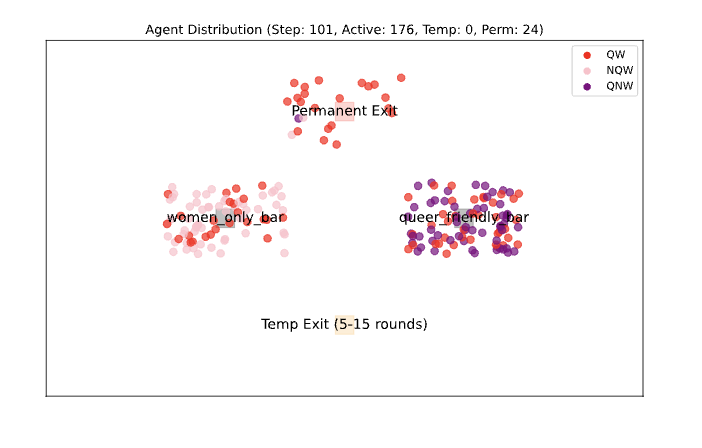
\includegraphics[width=\linewidth]{figures/0.5 bar.png}
  \caption{Agent Distribution of Simulation 1}
\end{minipage}
\hfill
\begin{minipage}{0.48\textwidth}
  \centering
  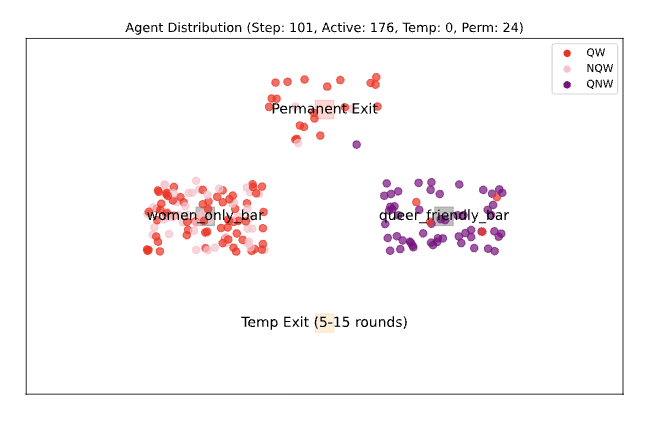
\includegraphics[width=\linewidth]{figures/0.5 bar 2.png}
  \caption{Agent Distribution of Simulation 2}
\end{minipage}
\end{figure}

\begin{figure}[H]
\centering
\begin{minipage}{0.48\textwidth}
  \centering
  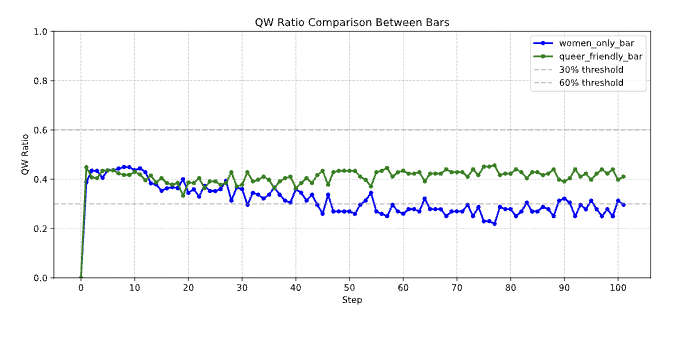
\includegraphics[width=\linewidth]{figures/0.5 ratio.png}
  \caption{QW Ratio Trends of Simulation 1}
\end{minipage}
\hfill
\begin{minipage}{0.48\textwidth}
  \centering
  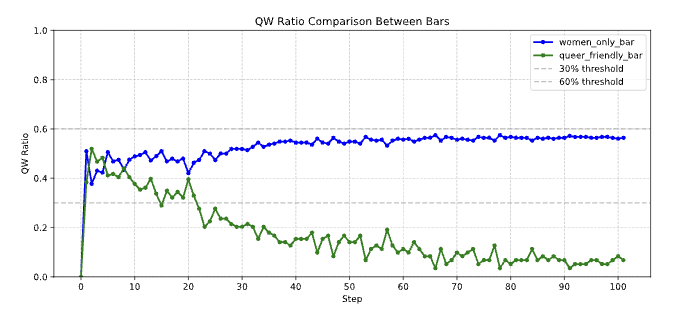
\includegraphics[width=\linewidth]{figures/0.5 ratio2.png}
  \caption{QW Ratio Trends of Simulation 2}
\end{minipage}
\end{figure}

\begin{figure}[H]
\centering
\begin{minipage}{0.48\textwidth}
  \centering
  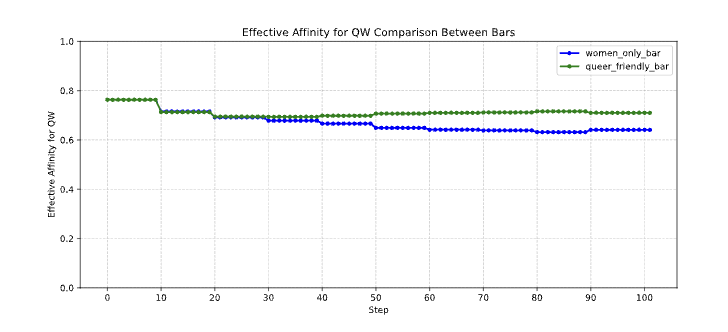
\includegraphics[width=\linewidth]{figures/0.5 ea.png}
  \caption{Effective Affinity of QW in Simulation 1}
\end{minipage}
\hfill
\begin{minipage}{0.48\textwidth}
  \centering
  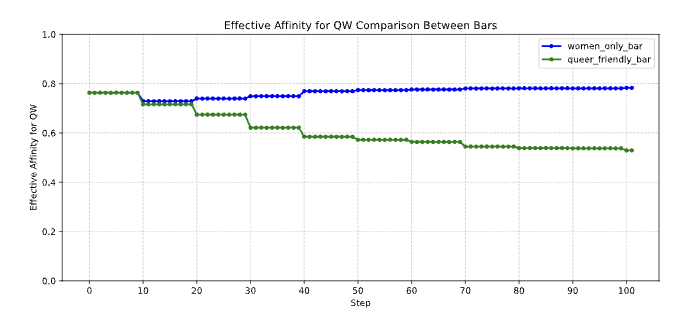
\includegraphics[width=\linewidth]{figures/0.5 ea2.png}
  \caption{Effective Affinity of QW in Simulation 2}
\end{minipage}
\end{figure}


In the first simulation (random seed = 42), the women-centered bar stabilized with a consistently high QW ratio and maintained a strong effective affinity for QW. The queer-centered bar, by contrast, experienced an early decline in QW ratio and a corresponding drop in affinity. This suggests that early demographic differences—perhaps driven by random fluctuation—may have triggered self-reinforcing feedback loops that favored one group over another.

In the second simulation (random seed = 929), the dynamic was reversed. The queer-centered bar sustained QW presence and alignment, while the woman-centered bar experienced gradual demographic drift and symbolic erosion. Together, these two cases illustrate that bar type does not deterministically produce cultural retention or loss. Instead, early fluctuations in attendance, amplified through institutional responsiveness, play a central role in shaping long-term outcomes.

This finding supports sociological accounts of path dependence in identity-based space \citep{podmore2006}. A bar’s fixed strategy establishes initial conditions, but the long-term symbolic identity of the space emerges through feedback: patterns of presence, withdrawal, and adaptation accumulate and self-reinforce. In this model, strategic labels serve as predispositions rather than guarantees.

\subsection{Social Adaptability and the Stability of Lesbian Identity}

While the first set of simulations examined the role of bar strategy, this section focuses on a second core parameter: $\gamma$ (gamma), which governs how responsive a bar is to recent patterns of attendance. Gamma controls the weight given to fixed versus adaptive affinity when agents compute their belonging score. A higher gamma means the bar relies more on its original strategic orientation; a lower gamma means the bar is more socially adaptable, updating its cultural tone more readily in response to recent visitors.

This parameter is of both theoretical and practical interest. In real-world LGBTQ+ nightlife, some venues maintain strong cultural boundaries even as social norms evolve, while others adjust their atmosphere rapidly to attract broader clientele. Gamma thus encodes a dimension of institutional flexibility versus cultural continuity, reflecting the tension between preserving lesbian specificity and accommodating shifting demographics.

To assess the effects of gamma, I compare two illustrative simulations at different gamma levels: 0.3 (high adaptability) and 0.7 (low adaptability). In both cases, the fixed affinity structures, group distributions, and all other global parameters are held constant. The goal is to observe how bars with different adaptive tendencies navigate the same social environment, and whether either extreme produces more stable identity outcomes.

\begin{figure}[H]
\centering
\begin{minipage}{0.48\textwidth}
  \centering
  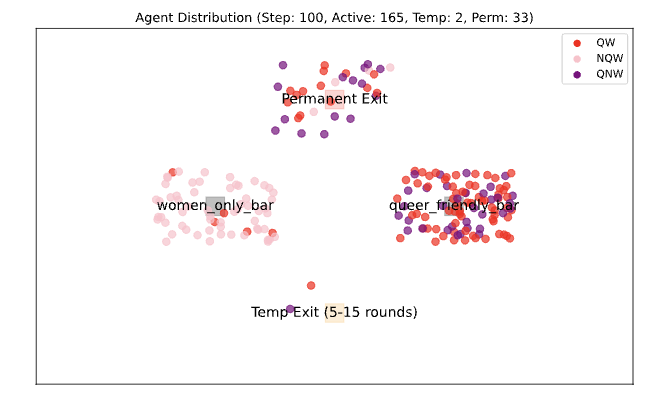
\includegraphics[width=\linewidth]{figures/0.3 bar.png}
  \caption{Agent Distribution($\gamma$ = 0.3)}
\end{minipage}
\hfill
\begin{minipage}{0.48\textwidth}
  \centering
  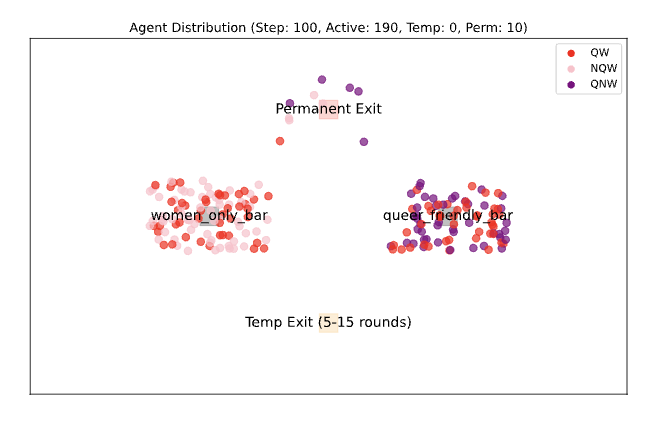
\includegraphics[width=\linewidth]{figures/0.7 bar.png}
  \caption{Agent Distribution($\gamma$ = 0.7)}
\end{minipage}
\end{figure}

\begin{figure}[H]
\centering
\begin{minipage}{0.48\textwidth}
  \centering
  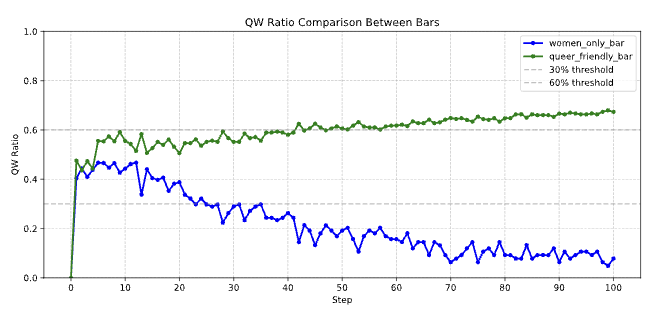
\includegraphics[width=\linewidth]{figures/0.3 ratio.png}
  \caption{QW Ratio Trends($\gamma$ = 0.3)}
\end{minipage}
\hfill
\begin{minipage}{0.48\textwidth}
  \centering
  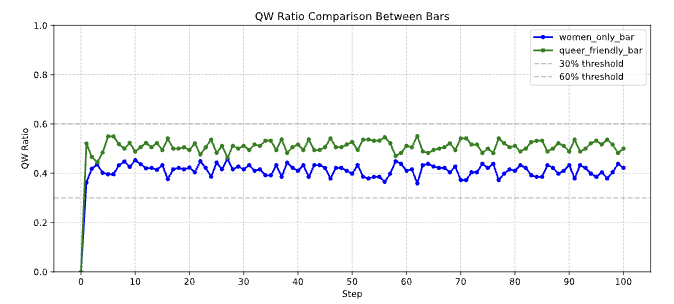
\includegraphics[width=\linewidth]{figures/0.7 ratio.png}
  \caption{QW Ratio Trends ($\gamma$ = 0.7)}
\end{minipage}
\end{figure}

\begin{figure}[H]
\centering
\begin{minipage}{0.48\textwidth}
  \centering
  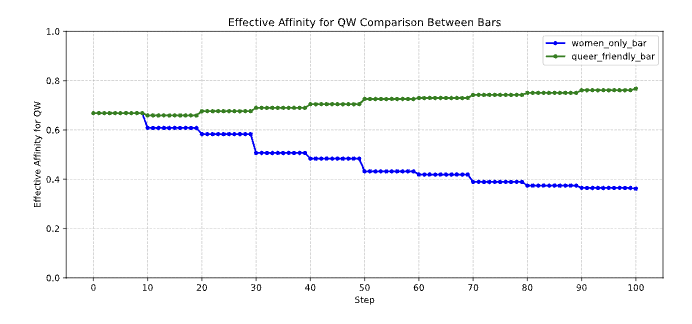
\includegraphics[width=\linewidth]{figures/0.3 ea.png}
  \caption{Effective Affinity of QW ($\gamma$ = 0.3)}
\end{minipage}
\hfill
\begin{minipage}{0.48\textwidth}
  \centering
  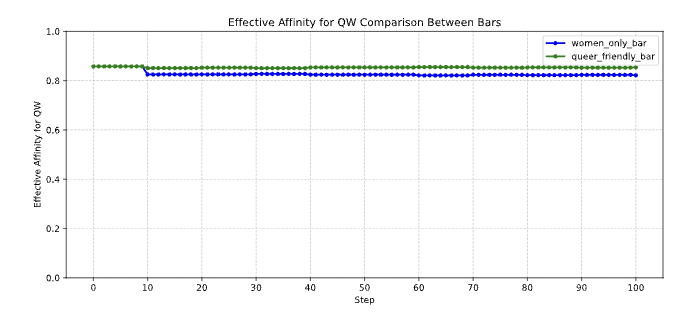
\includegraphics[width=\linewidth]{figures/0.7 ea.png}
  \caption{Effective Affinity of QW ($\gamma$ = 0.7)}
\end{minipage}
\end{figure}

In the simulation on the left($\gamma$ = 0.3), both bars rapidly adjust their adaptive affinities. As shown in Figure 9 and Figure 11, the QW ratio in the woman-centered bar steadily declines over time, falling below 0.2 by the end of the simulation. The corresponding effective affinity toward QW drops sharply (Figure 11), suggesting that the bar's cultural alignment has shifted in response to demographic change. Visual inspection of agent distribution (Figure 7) confirms this drift, with QW agents exiting or clustering around the queer-friendly bar instead.

In contrast, under $\gamma$ = 0.7, both bars remain much more culturally stable. The QW ratio stays within a narrower range (Figure 10), and effective affinity for QW remains consistently high in both spaces (Figure 12). As Figure 8 illustrates, agent distribution at step 100 shows well-maintained clustering around each bar, with limited QW withdrawal. These results suggest that higher gamma supports identity retention, at least within the range tested.

To assess the robustness of this pattern, we conducted batch simulations at $\gamma = 0.3$, $0.5$, and $0.7$, with 20 independent runs for each setting. The results are visualized in Figure~13 and Figure~14, which display the distribution of final QW population ratios and effective affinity scores across both bar types. These boxplots reveal a clear monotonic trend: as $\gamma$ increases—that is, as bars become less socially adaptive and more structurally fixed—both the retention of queer women (QW) and the cultural alignment with QW patrons tend to increase.


\begin{figure}[H]
\centering
\begin{minipage}{0.48\textwidth}
  \centering
  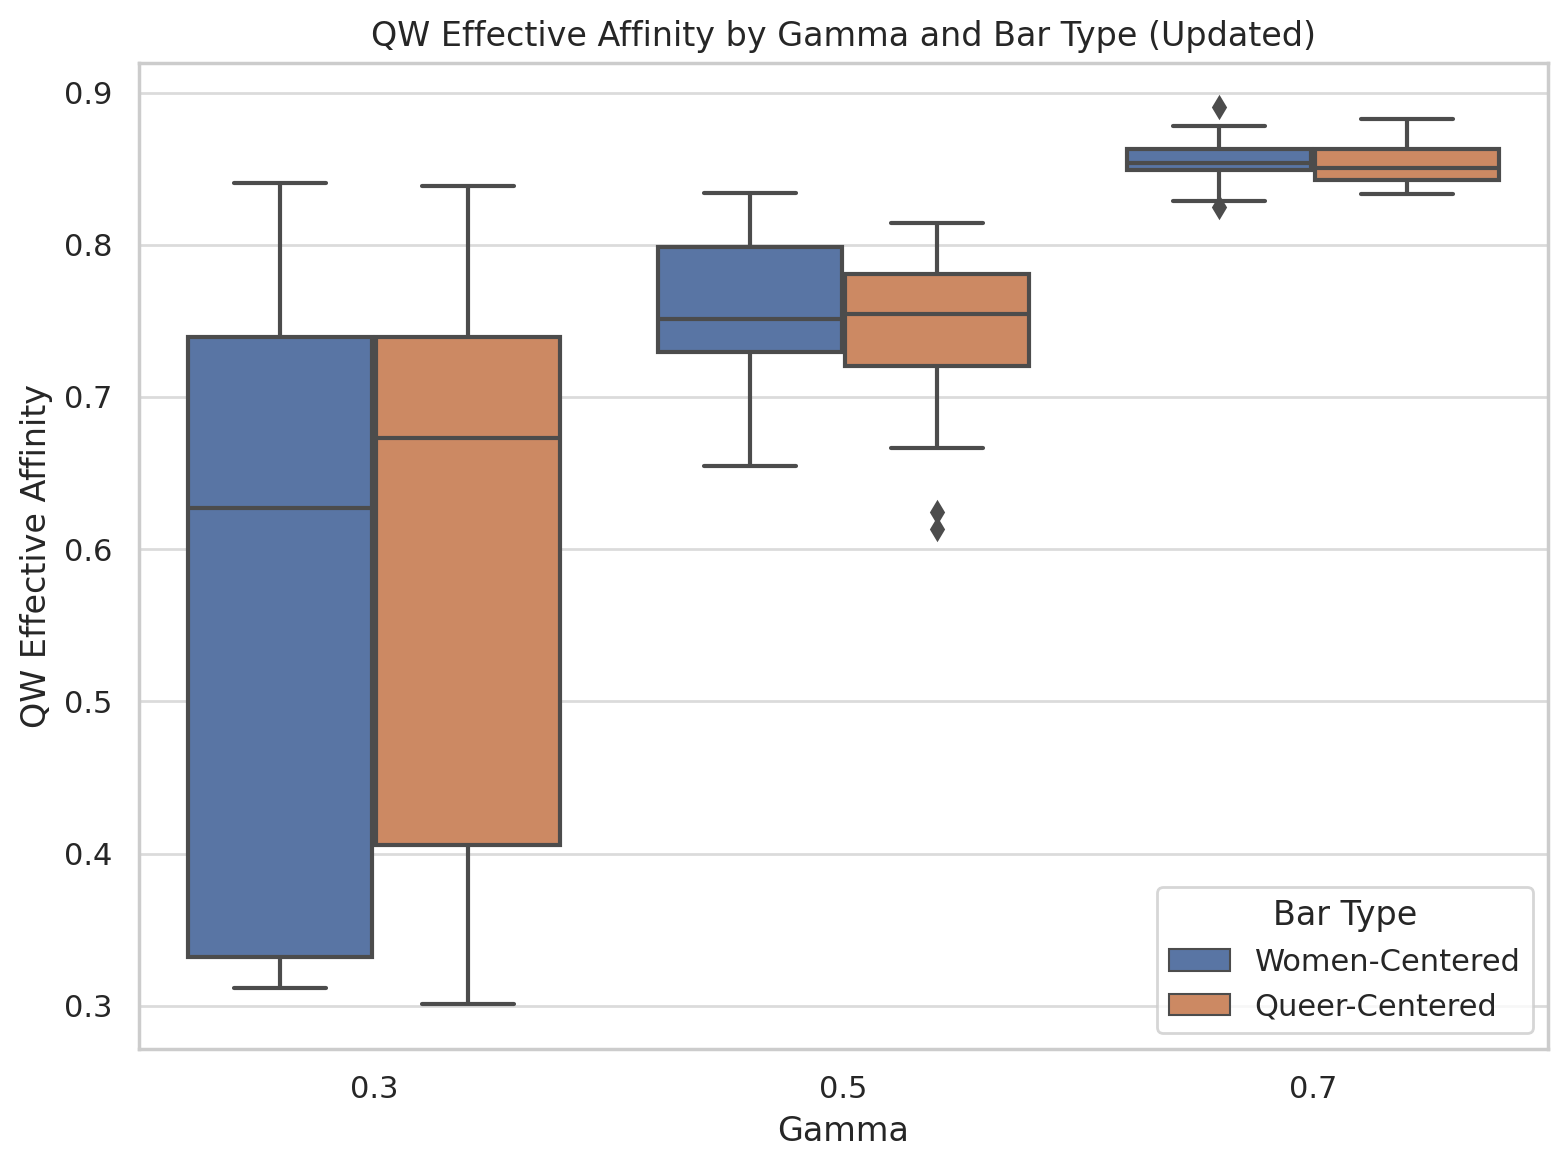
\includegraphics[width=\linewidth]{figures/batch ea.png}
  \caption{QW Effective Affinity by Gamma and Bar Type}
\end{minipage}
\hfill
\begin{minipage}{0.48\textwidth}
  \centering
  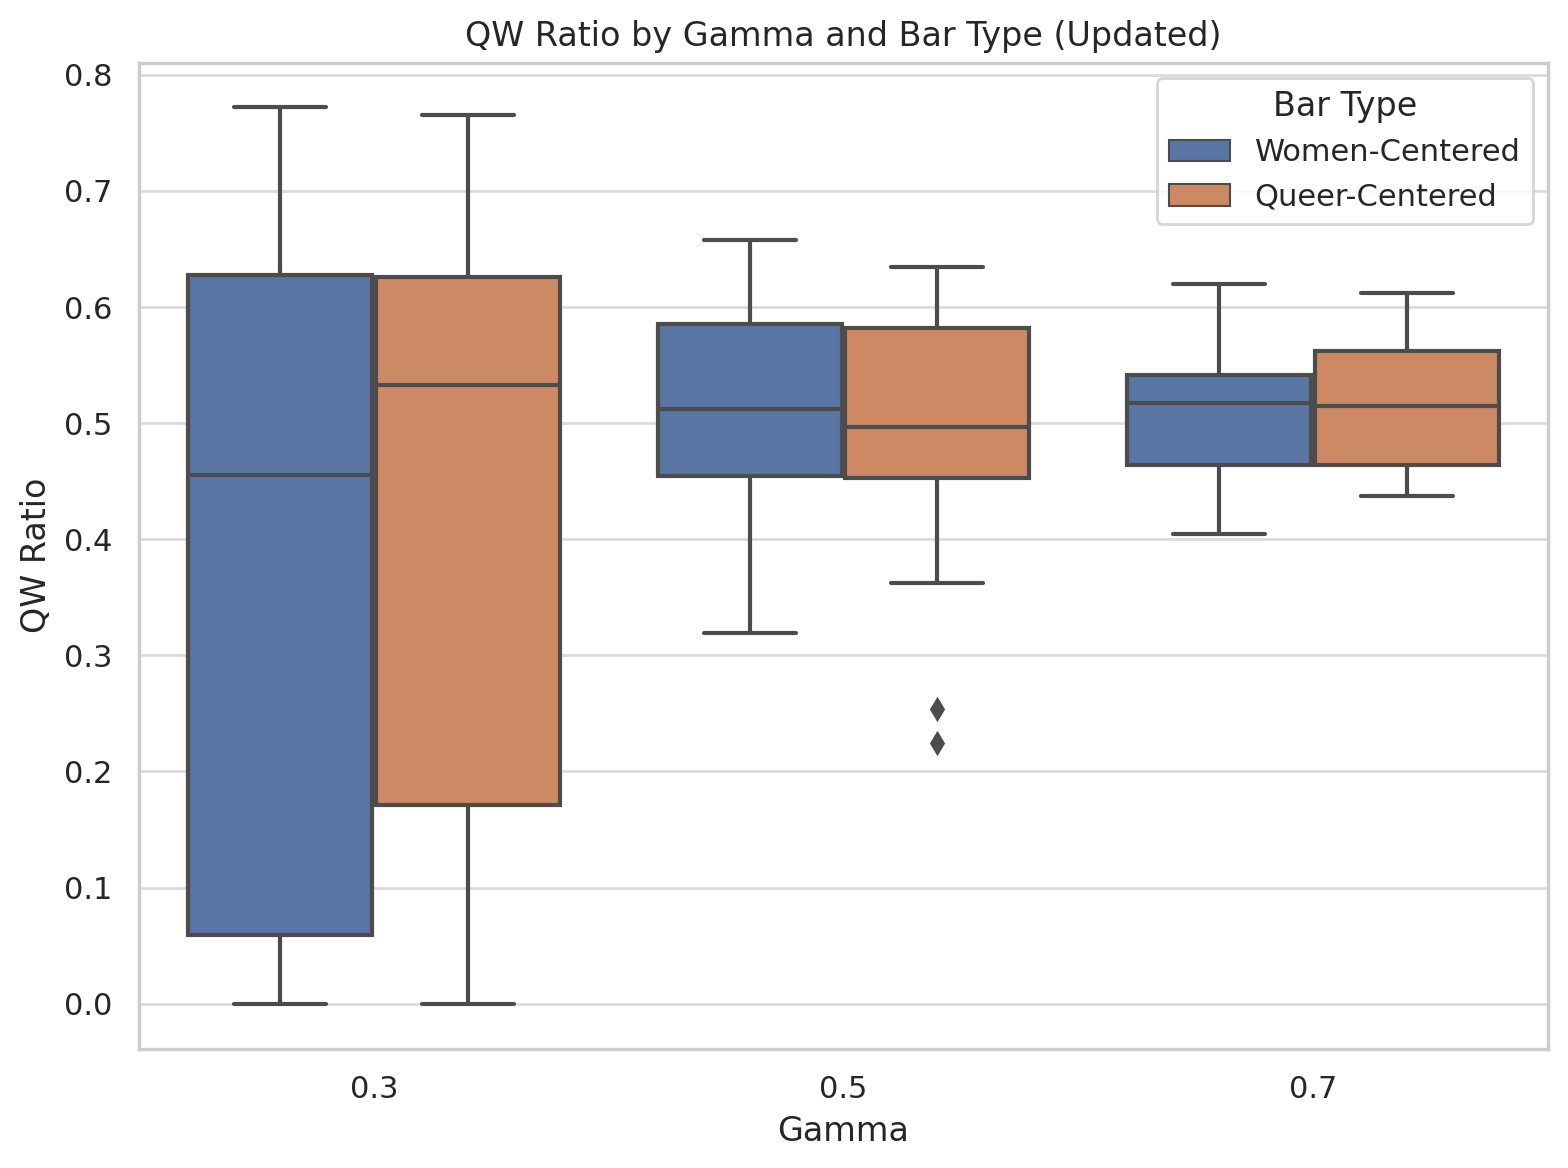
\includegraphics[width=\linewidth]{figures/batch ratio.png}
  \caption{QW Ratio by Gamma and Bar Type}
\end{minipage}
\end{figure}


At low adaptability levels ($\gamma = 0.3$), the QW ratio in queer-centered bars exhibits high volatility, with several runs showing near-zero presence, indicating severe identity drift. In contrast, higher $\gamma$ values produce more stable and elevated QW ratios in both bar types, with median values clustering around 0.5. A similar pattern holds for effective affinity scores: the distribution for $\gamma = 0.7$ is not only higher on average but also more tightly concentrated, suggesting stronger and more consistent symbolic alignment with QW participants.

Together, these visualizations reinforce the conclusion that institutional adaptability shapes the long-term cultural trajectory of lesbian bars. When bars rely more on fixed identity structures, they are better able to preserve symbolic coherence and demographic continuity. Rather than being driven by stochastic fluctuations in early attendance, the link between lower adaptability and stronger identity retention emerges as systematic, robust, and repeatable across simulations.

At the same time, some degree of responsiveness remains important: bars that entirely ignore recent participation patterns may risk becoming rigid or demographically misaligned. This trade-off between cultural stability and inclusiveness mirrors real-world debates about branding, belonging, and accountability in lesbian and queer nightlife. The parameter $\gamma$ provides a formal tool to explore these tensions, showing that the sustainability of identity-based space depends not only on who is allowed in, but also on how cultural signals are produced, interpreted, and revised over time.

\section{Discussion}

This paper developed an agent-based model to examine how strategic orientation and institutional adaptability influence the long-term demographic and cultural dynamics of lesbian bars. The analysis produced two main findings. First, a bar’s initial strategy—whether woman-centered or queer-centered—does not directly determine its cultural outcome. Instead, early fluctuations in attendance, when reinforced through feedback mechanisms, shape divergent trajectories. Second, the degree of institutional adaptability, operationalized by the gamma parameter, plays a substantial role in cultural stability. Bars with higher gamma values tend to maintain stronger alignment with their intended core group. In contrast, highly adaptive bars are more susceptible to shifts in identity composition.

These findings speak to broader questions in urban sociology and queer studies about how identity-based spaces respond to external and internal pressures. The model suggests that the symbolic identity of a space is not solely a product of fixed strategy or self-labeling, but emerges through ongoing interaction between institutional structure and community behavior.

Several limitations should be acknowledged. First, the analysis relies on a small number of illustrative simulation runs. While these runs help clarify possible mechanisms, they do not support claims about the generality or statistical significance of outcomes. Second, the parameter values used in the model, such as the intergroup preference matrix, population distribution, and belonging thresholds, are based on plausible assumptions informed by qualitative studies. However, these values remain subjective and are not directly drawn from empirical measurements. Third, the bars in the model are not strategic actors. They do not make active decisions or respond intentionally to demographic shifts. Instead, their behavior is entirely determined by feedback from recent attendance patterns. This limits the model’s ability to capture real-world processes such as rebranding, policy change, or selective inclusion and exclusion.

Future research could address these limitations by running systematic batch simulations, performing sensitivity analysis across a wider range of parameters, and integrating more institutionally active mechanisms. It may also be valuable to compare simulated results with qualitative or observational data from real lesbian and queer nightlife venues. More generally, this model offers a flexible structure for exploring how community spaces maintain, transform, or lose their symbolic identity in response to the cumulative effects of everyday participation.

\bibliographystyle{chicago} 
\bibliography{references}   

\end{document}